\section{Definitions} \label{chapter3:definitions}

The continuous growth and sustainability of a platform relies on three criteria.
This section defines these tree criteria, as well as all the underlying concepts.

% Additionally, for the context of this thesis, a fourth criterium appears in this list.
% It is important for the analyzed platforms to be web compliant.\nt{I don't know where to put this criterium}

\begin{itemize}
\item Productivity
\item Efficiency
\item Adoption
% \item Web compliance
\end{itemize}

\subsection{Productivity}

% Software productivity is defined as the degree to which a platform allows an application the created, and then can be understood, fixed, and extended.
The productivity of a platform is the degree to which developers can quickly produce new and modify existing software.
% For an application to be maintainable, it needs to be modular.
%Productivity relies on modularity.
For a platform to be productive, it needs to enforce modularity directly in the design of applications.
Productivity later leads to maintainability.
% For an application to be maintainable, its platform needs to be highly productive.
% It relies on two factors, module encapsulation and module composition.

\subsubsection{Modularity}

Modularity is about encapsulating subproblems and composing them to allow greater design to emerge.
It allows to limit the understanding required to contribute to a module \cite{Stevens1974}, which helps developers to repair and enhance the application. 
Additionally, it reduces development time by allowing several developers to simultaneously implement different modules \cite{Wong2009,Cataldo2006}.

The criteria to define modules to improve productivity are high cohesion and low coupling \cite{Stevens1974}.
Cohesion defines how strongly the features inside a module are related.
Coupling defines the strength of the interdependences between modules.
% Encapsulating a subproblem into a module helps increase cohesion.
% Composition abstractions helps decrease their coupling.
The encapsulation of modules helps increase their cohesion, and their composition helps decrease coupling.
Encapsulation and composition improve productivity.

\begin{itemize}
\item Encapsulation $\to$ High Cohesion
\item Composition $\to$ Low Coupling
\end{itemize}

\subsubsection{Encapsulation}

\paragraph{Boundary Definition}
\illustration{spaghetti programming}%
Modular Programming stands upon Structured Programming \cite{Dijkstra1970}.
% Dijkstra firstly developed the concept of Structured Programming \cite{Dijkstra1970}, which later led to modular programming.
% It is defined as \textit{the systematic use of abstraction to control a mass of details, and also a means of documentation which aids program design} \cite{Knuth1974}.
It draws clear interfaces around a piece of implementation so that the execution remains enclosed inside.
At a fine level, it helps avoid spaghetti code \cite{Dijkstra1968a}, and at a coarser level, it structures the implementation \cite{Dijkstra1968} into modules, or layers.
% The next paragraph explains further the criteria to draw the borders around modules.

\paragraph{Data Protection}
\illustration{lasagna programming}%
Modular programming encapsulates a specific design choice in each module, so that it is responsible for one and only one concern.
It isolates its evolution from impacting the rest of the implementation \cite{Parnas1972, Tarr1999, Hursch1995}.
Examples of such separation of concerns are the separation of the form and the content in HTML / CSS, or the OSI model for the network stack.

\subsubsection{Composition} \label{chapter3:software-productivity:modularity:features}

\paragraph{Higher-Order Programming}
% \nt{If possible, include this reference : Continuations and coroutines \cite{Haynes1984}}
% Higher-order programming 
Higher-order programming introduces lambda expressions, functions manipulable like any other primary value.
They can be stored in variables, or be passed as arguments.
It replaces the need for most modern object oriented programming design patterns \ftnt{http://stackoverflow.com/a/5797892/933670} with Inversion of Control \cite{Johnson}, the Hollywood Principle \cite{Sweet1985}, and Monads \cite{Wadler1992}.
Higher-order programming help loosen coupling, thus improve productivity \cite{Haynes1984}.

\paragraph{Closures}
In languages allowing mutable state, lambda expressions are implemented as closure, to preserve the lexical scope \cite{Sussman1998}.
A closure is the association of a function and a reference to the lexical context from its creation.
It allows this function to access variable from this context, even when invoked outside the scope of this context.
% \nt{next sentence is redundant with the suit}
% It eventually tangles the memory references so that it requires a global memory.

\paragraph{Lazy Evaluation}
% Lazy evaluation 
% Lazy evaluation is an evaluation strategy allowing to defer the execution of a function only when its result is needed.
Lazy evaluation allows to defer the execution of an expression when its result is needed.
The lazy evaluation of a list is equivalent to a stream with a null-sized buffer \cite{VanRoy2003}. %, while the opposite, eager evaluation, corresponds to an infinite buffer \cite{VanRoy2003}.
It is a powerful tool for structuring modular programs, as the execution is organized as a concurrent pipeline \cite{Sussman1983}.
The stages process independently each element of the stream.
But this concurrency requires the isolation of side-effects to avoid conflicts between stages executions.
% \nt{find another transition}Indeed, the dataflow programming paradigm resulting from lazy lists is particularly adapted for stream processing applications.

% \paragraph{Late Binding}

% Late binding allows to defer the resolution of references to the execution.
% It improves the composition.



\paragraph{}

The criteria to analyze the productivity of platforms are the following.
\begin{itemize}
\item Encapsulation $\to$ High Cohesion
  \subitem Boundary definition
  \subitem Data protection
\item Composition $\to$ Low Coupling
  \subitem Higher-order programming, Lambda Expressions
  \subitem Lazy evaluation, Stream composition
\end{itemize}


\subsection{Efficiency}

The efficiency of a software project is the relation between the usage made of available resources and the delivered performance.
For an application to perform efficiently, the platform based on needs to enforce scalability directly in its design.

Scalability relies on the parallelism allowed by the commutativity of operations execution \cite{Clements2013a}.
An operation is a sequence of statements.
Operations are commutative if the order of their executions is irrelevant for the correctness of their results.
Commutativity assures the independence of operations.

\subsubsection{Independence}

\illustration{Synchronization vs Message-passing}
The independence, and commutativity of an operations depends on its accesses to shared state.
If the operations doesn't rely on any shared state, it is independent.
The independence of operations allows to execute them in parallel, hence to increase performance proportionally to occupied resources \cite{Amdahl1967,Gunther1993}.
But if they rely on shared state, they need to coordinate the causal scheduling and atomicity of their executions to avoid conflicting accesses.
This scheduling between the operations can be defined in two ways.
\begin{description}
\item[Synchronization] Operations are scheduled sequentially to have the exclusivity on a shared state, or
\item[Message-passing] Operations communicate their local modifications of the state to other operations, in a decentralized fashion.
\end{description}

\subsubsection{Atomicity}

An operation is atomic if it happens in a single bulk.
The beginning and end are indistinguishable for an external observer.
% The causality between the operations, in conjunction with exclusivity, assures the atomicity of the memory accesses.
It assures the developer of the invariance of the memory during the operation.
It relies either on the causal scheduling of operations -- synchronization -- or exclusivity of their memory accesses -- message-passing.
% In other words, either operations are executed one after the other, or they access different memory regions.

\subsubsection{Granularity}

If the operations access the state too frequently, the communication overhead of message passing exceeds the performance gains of parallelism.
And if operations access the state too rarely, the synchronization required for sharing state limits the possible parallelism.
These two extremes are inefficient.
% Efficiency relies on a compromise between the two.
% the centralization of the state limits the parallelism.
% Additionally, because of the latency of the web, synchronization between remote locations obliterates performance.
Operations tend to share state closely at a fine-grain level and less at a coarser-grain level.
% Therefore, at a fine-grain level the operations need to be scheduled sequentially to avoid the communication overhead.
% And at a coarse-grain level they need to communicate via message-passing, to allow parallelism.
Therefore, efficiency requires the combination of fine-level state sharing to avoid communication overhead, and coarse-level independence to allow parallelization \cite{Gustafson1988,Gunther1996,Nelson1996,Gunther2002}.
The threshold determining frequent or rare access to the state determines the granularity level between synchronization and parallelization of tasks.

\paragraph{}

The criteria to analyze the performance of platforms are the following.

\begin{itemize}
\item Fine-level state sharing
  \subitem State mutability $\to$ Synchronization
\item Coarse-level independence
  \subitem State immutability $\to$ Message-passing
\end{itemize}

% \subsubsection{Event-Loop Execution Model} \label{chapter2:web-as-a-platform:javascript:event-loop}

% \nt{Reduce the event-loop explanation to the bare minimum, the definitions of callbacks and promises should be in the state of the art. It only need to present briefly how the event-loop works to understand the problem}

% Javascript is often associated with an event-based paradigm to react to concurrent user interactions.
% In 2009, Joyent released Node.js to build real-time web services with this paradigm.
% It is a server-side implementation of Javascript based on an event-loop.
% This event-based paradigm proved to be very efficient as well for a web service to react to concurrent requests.
% This section presents the event-loop execution model, and the advantages of Javascript for this paradigm.

% The event-loop efficiency comes from non-blocking communications, asynchronous execution, and cooperative scheduling.
% It relies on a queue storing the messages received asynchronously.
% The loop executes tasks previously defined to process these messages one after the other.
% Each task can initiate new communications, leading in turn to the queuing of more messages, which trigger more tasks, and so on.
% Each task is executed atomically and exclusively, until it yields execution to continue with the next task in queue.

% \nt{TODO schema of an event-loop}

% \paragraph{Callbacks}

% In Javascript, the asynchronous communications are initiated by function calls.
% The callee immediately returns to avoid the caller to wait for the result.
% The task to process the result of the communication, and to continue the execution afterward, is a function passed as an argument to the callee.
% This function is named a callback or a continuation.
% A callback is a function passed as an argument to a callee.
% It is a continuation if the callee calls it to transfer the control back to the caller without the need for synchronization.

% In this execution model, the control flow follows the asynchronous function calls and callbacks.
% It organizes the execution of callbacks causally, one after the other, similarly to a pipeline.
% Indeed, the input stream of data flows through a sequence of callbacks until the application outputs it.
% In this model, callbacks are the atoms of the asynchronous execution flow control.
% The next paragraph presents a more elaborate form of control.

% \paragraph{Promises}

% Since the asynchronous execution flow became more complicated on larger web application, many projects proposed improved asynchronous execution controls on top of callbacks.
% The ECMAScript specification proposes Promises for such purpose.
% It arranges sequences of causally related callbacks into cleanly organized pipelines of callbacks communicating their results to the next.

% \paragraph{Closures}

% Because callbacks can be passed as an argument, they are first class citizen and imply higher-order programming. %, which is part of functional programming.
% % Javascript features higher-order functions.
% For a callback to continue the execution without needing synchronization with the caller, it needs to have access to the initial context of the caller.
% This context is linked with the function when passed to the callee.
% The association of a function and its initial context is called a closure.

% Higher-order programming is convenient for developers, as they allow great modularity in the implementation through \textit{e.g.} inversion of control.
% It is presented in further details in section \ref{chapter3:software-productivity}.
% However, because the contexts are passed, and shared all over the implementation, this programming model needs a global memory for coordination.
% A global memory is problematic to increase the concurrency of the execution.

% This section presented Javascript as the language of the web, and its programming model.
% The next section presents the realities and technical challenges to assure the performance of web services against billions of users.






\subsection{Adoption}

An application is sustainable only if the platform used to build it generates reinforcing interactions between a community of passionate and the industry.
A platform needs to present a balance between productivity and efficiency to be adopted by both the community and the industry.
The productivity is required for a platform to be appealing to gather a community to support the ecosystem around it.
And the efficiency is required to be economically viable and needed by the industry, and to provide the reason for this ecosystem to exist.
Additionally, the web acts as a tremendous catalyst fueling these interactions.

\paragraph{}

The criteria to analyze the adoption of platforms are the following.

\begin{itemize}
\item Community Support
\item Industrial Need
\end{itemize}

\paragraph{}

Adoption requires a balance between efficiency and productivity.
% The granularity of execution needs to be free from the decomposition into modules.
% If the too are related, they interfere with each other, and impact either productivity, or efficiency.
This incentive to balance between productivity and efficiency is illustrated in figure \ref{fig:state-of-the-art}.
This figure is used throughout this chapter to graphically represent all the platforms analyzed.

\begin{figure}[h!]
\begin{center}
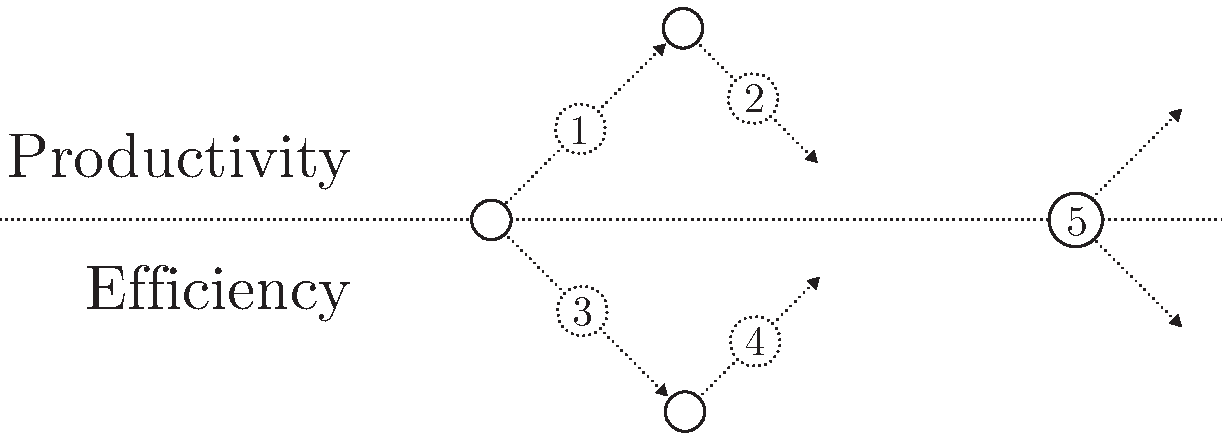
\includegraphics[width=0.6\textwidth]{../ressources/state-of-the-art.pdf}
\end{center}
\caption{Balance between Efficiency and Productivity}
\label{fig:state-of-the-art}
\end{figure}


% \subsection{Web}




% Pour la justification Web, je pense que tu dois raisonner que c'est le seul marché réellement explosif, donc c'est celui que tu vises. 

% Il y a pas mal d'arguments pour cibler le web :
% - technologies assez peu connues, car souvent imaginées comme n'étant qu'un problème d'ihm,
% - omniprésence sur internet,
% - et comme tout business doit passer par Internet, il faut comprendre le web en priorité. 

% Ne bloque pas trop sur le Web, pour moi c'est le contexte de fond, donc il faut que les plateformes soient orientées web. Je pense qu'un autre argument lié au web, c'est celui de TCP/IP, c'est à dire que les plateformes doivent accepter le délais dans les échanges. 